\chapter{Indledning}
I dette projekt er der arbejdet med design og udvikling af et blodtryksmålersystem. Ideen bag vores system blev udtænkt og udarbejdet med viden om en blodtryksmåler på en operationsstue på Herning Sygehus. Vores opstillede krav samt design til systemet, blev derfor lavet ud fra de oplysninger vi fik af en sygeplejerske\footnote{Anæstesi sygeplejerske Charlotte Høj, Herning Sygehus} på Herning Sygehus. Der var et ønske om at lave et blodtryksmålersystem, som er så virkelighedsnært som muligt. Det design og de funktionaliteter der blev efterstræbt i dette projekt var derfor at præsentere et blodtrykssignal, hvor det systoliske samt det diastoliske blodtryk kan bestemmes, få præsenteret et EKG-signal, hvorfra pulsen kan bestemmes, og præsentere iltmætningen i blodet, for patienten. Ud fra de ønskede funktionaliteter ønskedes det at få implementeret og hermed få grafer og værdier vist på en brugergrænseflade, som lever op til de standarder, der ses på operationsstuer i dag. \\
\\
Baggrunden for dette projekt er, at man i klinisk praksis har behov for kontinuert at observerer patientens blodtryk. Det er i særdeleshed på intensiv afdelinger og operationsstuer, at man ønsker at lave direkte invasiv blodtryksmåling. Ved invasiv blodtryksmåling kan man monitorere patientens fysiske tilstand under eksempelvis en operation. Blodtrykket kan give en indikation om blødning, smerter og hvor dybt patienten sover under narkosen. Denne overvågning giver det sundhedsfaglige personale en ekstra tryghed og sikkerhed om patientens tilstand under operation. \\
\\
Denne projektrapport vil give en kort beskrivelse af vores samlede system samt krav hertil. Der vil være en udspecificeret projektbeskrivelse, som vil give et indblik i vores vej frem til det endelige resultat, og som også vil beskrive både de til- og fravalg vi har måttet tage, for at nå frem til netop det system vi ønskede at realisere og præsentere. Der har i den forbindelse været nogle ideer og ønsker, som ikke har været realistiske og tidsmæssigt mulige at opfylde og vil derfor være beskrevet i fremtidigt arbejde. Slutteligt vil derfor være en samlet konklusion på projektarbejdet.
\chapter{Projektformulering og afgrænsning}
I dette projekt ønskes der at udarbejde et produkt, der kan måle blodtrykket for en patient og vise dette løbende på en graf. Desuden skal produktet kunne bestemme det diastoliske tryk og det systoliske tryk ud fra blodtrykskurven og ud fra disse trykværdier bestemme middeltrykket. Ud fra systolisk og diastolisk tryk skal produktet kunne vise om en eller begge er overskredet en grænseværdi og signalere dette til det sundhedsfaglige personale. Produktet skal kunne filtrere det indhentede signal, med et digitalt filter, sådan at signalet kan vises filtreret og ufiltreret.  \\\\
Dette betyder at produktet skal kunne:
\begin{itemize}
\item Indhente et blodtrykssignal igennem hardwaren, hvilken består af:
\begin{itemize}
\item Væskefyldt kateter
\item Transducer 
\item Forstærker
\item Lavpas filter
\item NI-DAQ
\end{itemize}
\item Vise blodtrykskurven kontinuert
\item Vise blodtrykskurven både filtreret og ufiltreret
\item Bestemme systolisk tryk
\item Bestemme diastolisk tryk
\item Bestemme middeltryk
\item Starte alarm hvis systolisk/diastolisk tryk har overskredet en grænseværdi
\item Gemme patientens data i en database
\end{itemize}
Løsningen til dette produkt har for vores vedkommende været et software og et hardware produkt, hvilke benyttes sammen til at indhente, behandle og vise blodtrykssignalet. Hardwaren bruges til at indhente og behandle blodtrykssignalet, sådan at dette signal kan indsendes til softwaren. Softwaren skal kunne viderebehandle signalet, sådan at det indlæste signal kan præsenteres på en korrekt måde. Softwaren skal have en brugergrænseflade, hvilken bruges til at præsentere blodtrykssignalet for det sundhedsfaglige personale. \\
Ligeledes er det er ønske at produktet indhente EKG-signalet for patienten, samt iltsaturationskurven. Disse data skal også kunne vises på brugergrænsefladen. Ud fra EKG-signalet bestemmes pulsen, altså hjertefrekvensen for patienten, pulsen kan dog også bestemmes ved at finde antallet af systoliske værdier pr. minut, denne værdi præsenteres som talværdi på brugergrænsefladen. Ud fra iltsaturationskurven kan iltmætningen for blodet bestemmes, hvilken lideledes præsenteres på brugergrænsefladen. 
\section{Oversigt over projektdeltagere og hovedansvarsområder}
I dette projekt er det valgt at dele projektets deltagere op i to grupper med hver deres hovedansvarsområder. Den ene gruppe har beskæftiget sig med hardware og den anden gruppe har beskæftiget sig med software. Derudover blev der i starten af forløbet blev der valgt en projektleder, hvis opgaver bestod i at lave dagsorden for hvert møde, sørge for at deadlines blev overholdt, træffe endelige beslutninger og holde et overordnet overblik over projektet. En procesleder blev ligeledes valgt, hvis opgaver bestod i opgavestyring, godt arbejdsmiljø i gruppen og planlægning af projektforløbet. \\
Herunder ses de forskellige gruppemedlemmers hovedområde.\\\\
\begin{tabular}{| l | l |} \hline
\textbf{Hardware} & \textbf{Software}\\\hline
Brian Hansen & Ida Mark Skovbjerg \\\hline 
Mohamed Hussein Mohamed & Mette Østergård Knudsen \\\hline
Khaled Edwan & Line Skov Larsen  \\\hline 
\end{tabular}
\\\\
Gruppens medlemmer med fulde navn og initialer ses herunder, det er initialerne benyttes som reference til gruppemedlemmerne herfra. \\\\
\begin{tabular}{| l | l |} \hline
\textbf{Fulde navn} & \textbf{Initialer}\\\hline
Ida Mark Skovbjerg & IMS \\\hline 
Line Skov Larsen & LL \\\hline
Mette Østergård Knudsen & MK  \\\hline 
Brian Hansen & BH \\\hline
Mohamed Hussein Mohamed & MM \\\hline 
Khaled Edwan & KE \\\hline
\end{tabular}
\chapter{Hjertet - en muskel}
Hjertet er en muskel, der fungerer som en pumpe i kroppen. Hjertet pumper det iltede blod (arterielt blod) ud til resten af kroppen gennem arterie- og vene systemer. Når blodet passerer ud af hjertet igennem arterierne sker der et tryk mod arterievæggene, dette tryk kaldes blodtrykket. \\\\
Hjertet opdeles i to adskilte hjertehalvdele, som fungere som pumper. Den venstre, som pumper blodet rundt i organismen og den højre, som pumper blodet gennem lungerne. De to hjertehalvdele er sammensat af atrium og ventrikler. Blodet fra organismen der føres tilbage til hjertet, er det venøse blod, som føres tilbage til højre atrium gennem øvre og nedre hulvene. Mellem højre atrium og højre ventrikel sidder trikuspidalklappen, som forhindrer blodet i at løbe tilbage til atriet under hjertets sammentrækning. Fra højre ventrikel udløber i lungepulsåren, som deles ud i hver lunge. Mellem ventriklen og lungepulsåren er pulmonalklappen, som forhindrer blodet i tilbageløb. I lungerne afgiver blodet CO$_{2}$ og optager ilt, denne diffusion af disse gasser sker i lungernes alveoler. Det nu iltrige blod returneres gennem lungevenerne til venstre atrium. Fra venstre atrium til venstre ventrikel sidder mitralklappen. Fra venstre ventrikel pumpes blodet ud i aorta gennem aortaklappen, herfra pumpes blodet rundt i resten af organismen. \cite{hjertedsd}
\begin{figure}[H]
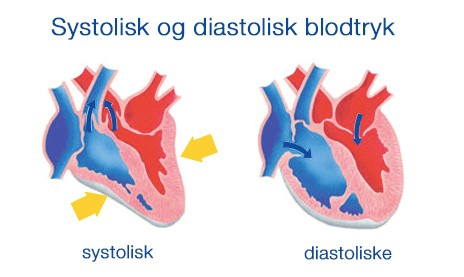
\includegraphics[width =0.5\textwidth , center]{billeder/sysdia}
\caption{\textbf{Her ses hjertet ved systoliske og diastoliske blodtryk.}}
\end{figure}
\section{Blodtryk}
Blodtrykket er trykket i blodkarrene, når blodet pumpes rundt i kroppen. Dette tryk sker, når hjertets venstre hjertekammer trækker sig sammen og der, som resultat heraf, bliver presset blod ud i arterierne. Trykket vil altså være størst i arterierne, da arterierne er de blodåre som fører væk fra hjertet. Det laveste blodtryk vil være at se i venerne, da det er de blodårer som fører blodet tilbage til hjertet. Blodtrykket vises som to værdier: systolen, som er hjertets sammentrækningsfase og diastolen som er hjertets afslapningsfase. \\\\
Systolen angives som den kraft, der skabes når der kommer pres på karvæggen i arterierne. Dette sker i hjertets sammentrækningsfase, hvor blodet pumpes ud i arterierne. Systolen i et normalt blodtryk i hvile vil ligge i intervallet 100-140mmHg og ved forhøjet blodtryk er værdien for trykket over 140 mmHg.\\ Diastolen angiver hjertets hvilefase og ses mellem to sammentrækninger. I denne fase fyldes ventriklerne med blod. Den normale værdi for diastolen ligger i intervallet 60-90 mmHg. Hvis den overstiger 90 mm Hg anses blodtrykket for at være forhøjet. Udover systolen og diastolen kan også middeltrykket angives. Denne udregnes ved $\dfrac{2}{3}\cdot Diastole + \dfrac{1}{3}\cdot Systole$ \cite{blodtrykwiki}
Hypertension defineres som forhøjet systole, forhøjet diastole eller både forhøjet systole og diastole. Hypertension belaster hjertet, og medføre en øget risiko for udviklingen af apopleksi. Det er også forbundet med flere medicinske tilstande såsom arteriosklerose, hjerteinsufficiens og nyreskader. \cite{pulmonal}\\
Hvis værdien for systolen kommer under 100 mmHg og/eller diastolen kommer under 60 mmHg, vil der være tale om et for lavt blodtryk, hypotension. Lavt blodtryk behøver dog ikke at være alvorligt, men kan være helt normalt for f.eks. høje personer. Men i forbindelse med sygdom, traumer eller medicinoverdosering er hypotension en alvorlig tilstand. Hypotension ses bl.a. ved diabetes, traumer, hjertesvigt og Addisons sygdom. \cite{hypo}
\\\\
Anatomien bag blodtrykket og blodtryksændring, omfatter blodets kredsløb, hjertet og lymfesystemet, som er kredsløbssystemet. Blodkredsløbet er et langt netværk af arterier og vener, som har til opgave at føre iltet blod ud til hver celle i kroppen, samt opfange affaldsprodukter fra celler og væv.\cite{pulmonal}  I lungekredsløbet udskilles affaldsprodukter og blodet iltes. Det er hjertet der pumper blodet ud i dette netværk, så blodet hele tiden er i bevægelse. Arterierne transportere blodet væk fra hjertet, og venernes opgave er at transportere blodet mod hjertet. 
\begin{figure}[H]
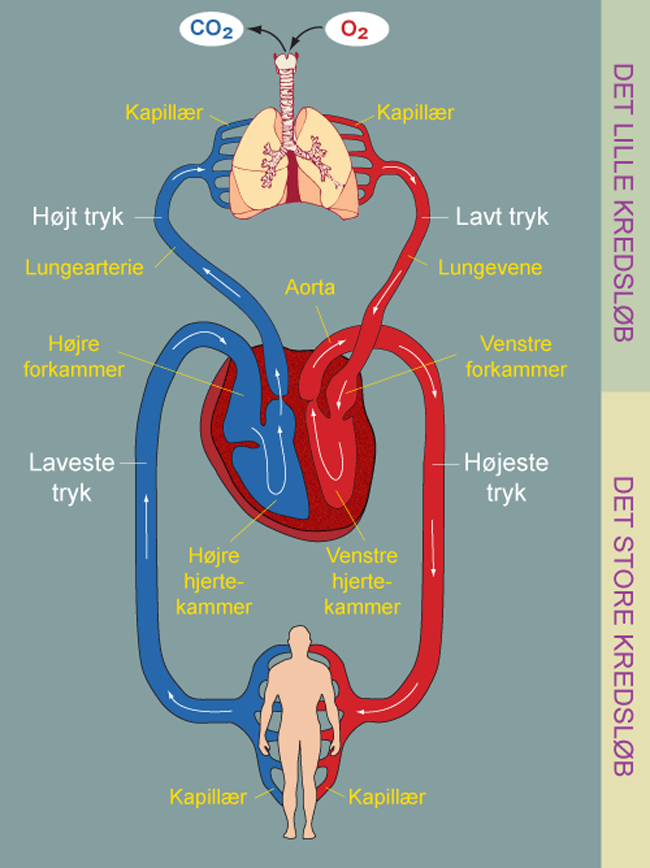
\includegraphics[width =0.5\textwidth , center]{billeder/hjertet}
\caption{\textbf{Det lille og det store kredsløb. Motoren der driver det hele er hjertet. \cite{hjertet}}}
\end{figure}
Kredsløbet kan funktionelt og anatomisk inddeles i to dele: Det pulmonale kredsløb og det systemiske kredsløb.\\
De to kredsløb fungerer i symbiose mellem hjertets højre hjertekamre og hjertets venstre hjertekamre. Højre siden pumper blodet gennem det pulmonale kredsløb, og venstre side pumper blodet rundt i det systemiske kredsløb.\\
Det pulmonale kredsløbs primære funktion er at levere blodet til lungekredsløbet, hvor blodet iltes. Hjertets højre side modtager iltfattigt blod og CO$_{2}$-rigt blod via v. Cava superior og inferior fra det systemiske kredsløb og pumper det videre ind i lungekredsløbet gennem det pulmonale kredsløb via pulmonal aterierne. Fra lungerne løber det nu iltrige og CO$_{2}$-fattige blod tilbage til venstre side af hjertet, som derfra pumper blodet videre til det systemiske kredsløb via aorta. \cite{pulmonal} 
\section{Direkte invasiv måling af blodtryk}
Den mest almindelig metode til klinisk at måle blodtrykket er ved at koble det vaskulære tryk til en extravaskulær sensor via et væskefyldt kateter. Klinisk er dette system påsat patientens a. Radialies via en arteriekanyle. Kateterslangen er forbundet til en trevejs stophane og videre til tryk sensoren. Kateter-sensor systemet er fyldt med en saltvandsopløsning fra væskesøjlen. Denne saltvandsopløsning skal skylle cirka hvert andet minut gennem systemet, dette forhindrer blodet i at størkne på spidsen.
\begin{figure}[H]
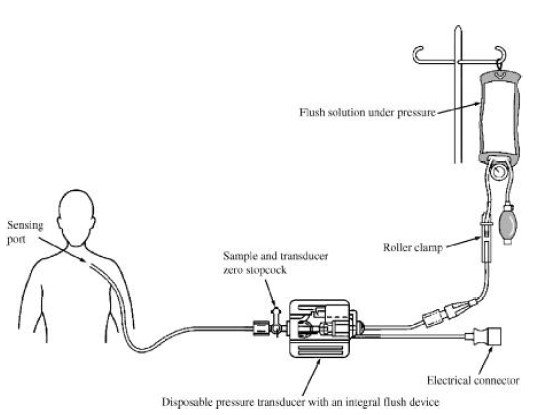
\includegraphics[width =0.7\textwidth , center]{billeder/kateter}
\caption{\textbf{Opstilling af direkte invasiv blodtryksmåling}}
\end{figure}
Som det ses på figuren er sansningsporten indgangen til patients arterie. Kateteret er koblet til trevejs stophanen og videre til sensoren. Trevejs stophanen har tre mulige funktioner, 1: Der kan lukkes for blodtilførslen så der er åbent for atmosfærisk luft og transduceren, dette giver værdien til nulpunktsjustering. 2: Der kan åbnes for atmosfærisk tryk ind til blodåren, dette kan bruges hvis patienten skal modtage medicin. Her indsættes medicin og ved at åbne for trykket fra væskesøjlen, vil medicinen flyde med blodet ind i blodåren. 3: Der åbnes for blodtilførsel ind i transduceren, dette giver blodtrykket. Blodtrykket transmitteres via kateter væskesøjlen ind i sensoren og til sidst i membranen. Det er her blodtrykket bliver målt. 
\chapter{Systembeskrivelse}
Det er blevet besluttet ud fra projektformuleringen at udvikle et blodtryksmålersystem som en prototype med perspektivering til fremtidigt arbejde. Blodtryksmålersystemet ønskes ideelt at kunne måle blodtryk, EKG og iltmætning for en patient. Ud fra blodtrykket findes systolisk og diastolisk blodtryk og udfra disse værdier kan middeltrykket bestemme. Systole og diastole bestemmes ved at finde den maksimale værdi (systole) og den minimale værdi (diastole) for blodtrykskurven. Middeltrykket herefter med formlen: $middeltryk = 1/3 \cdot systole + 2/3 \cdot diastole$. \cite{blodtrykwiki}
\\ Ud fra EKG-signalet kan pulsen bestemmes, dette gøres ved at bestemme antallet af R-takker på et minut. Desuden kan pulsen bestemmes ud fra blodtrykket, da pulsen her er antallet af systoliske værdier på et minut. Iltmætningen er mængden af ilt i blodet. For at kunne bestemme denne værdi skal et eksternt produkt benyttes. Dette produkt skal ved hjælp en infrarød sensor bestemme iltmætningen i blodet, dette bliver ikke implementeret i denne prototype.\\\\
Forudsætninger for brug af systemet er, at det skal køres på en computer, samt overholde de opstillede krav. Systemet er opbygget af en hardwaredel og en softwaredel. \\
Hardwaredelen består af et aktivt 2. Ordens Butterworth Sallen-Key lavpasfilter, samt en forstærker. Forstærkeren modtager et signal fra den udleverede transducer, dette signal forstærkes op. Signalet sendes videre til lavpasfilteret, hvor alle frekvenser over 50 Hz bliver dæmpet. Her fra sendes signalet ind i dataopsamlingsenheden NI-DAQ.\\\\
Softwaredelen består af et windows forms program udviklet i C\# .net, programmet skal kunne præsentere data indhentet fra DAQ’en. Ligeledes skal programmet kunne analysere og filtrere data fra DAQ’en, samt gemme disse i en "EPJ"-database. Programmet skal også kunne hente login-oplysninger fra en "personale"-database. \\
Man har valgt at have to databaser for at simulere det, at der er en adskillelse af medarbejderdata og patientdata.
\begin{figure}[H]
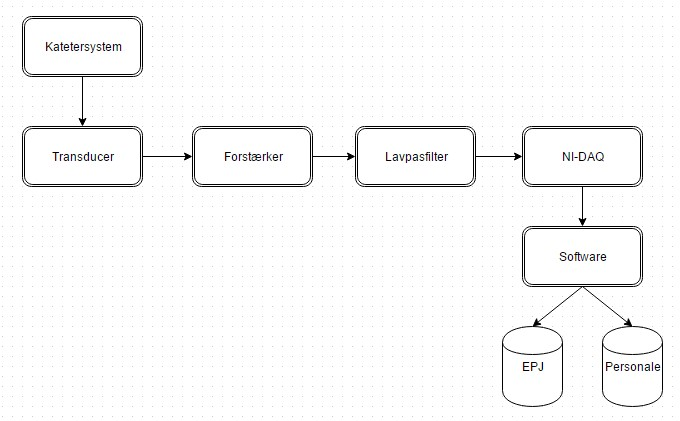
\includegraphics[width =0.8\textwidth , center]{billeder/system}
\caption{\textbf{Skitse af opbygning af systemet.}}
\end{figure}
\chapter{Krav}
Hvilke krav der stilles til produktet udarbejdes i en kravspecifikation. Denne kravspecifikation består af en række Use cases. Disse Use cases beskriver interaktionen mellem aktørerne og systemet. Use cases har til formål at specificere, hvilke krav der stilles til produktet. Kravene opstilles ud fra, hvad kunden ønsker, samt hvad leverandøren finder muligt at realisere. \\ \\
Der er nogle obligatoriske krav til produktet, der skal opfyldes. Disse krav er bl.a at systemet skal kunne kalibrere det indhentede blodtrykssignal og foretage en nulpunkts justering. Desuden skal blodtrykssignalet vises kontinuerligt, hvilket betyder, at signalet skal vises grafisk samtidigt med at det bliver hentet/indsendt fra hardwaren. Disse behandlede data skal desuden gemmes i en database.
Et af de obligatoriske krav er desuden, at der skal være et digitalt filter, der kan slås til og fra når programmet kører. Dette filter skal både kunne slås til og fra. Dette filter skal sørge for at signalet haves i to forskellige modes; et diagnose mode, hvor signalet er råt med alle udsving, og et monitor mode, hvor signalet er filtreret og afrundet.\\\\
Foruden disse obligatoriske krav er det valgt, at det skal være muligt at starte og stoppe målingen. Når målingen er startet skal det være muligt at justere grænseværdierne for systolen og diastolen, så grænseværdierne kan tilpasses patienten. Når signalets værdier overskrider en af grænseværdierne, skal en alarmering begynde. Denne alarm skal kunne udsættes i et minut, dog kun alarmens lyd, så det stadig er tydeligt at en grænseværdi der er overskredet.\\
Systemet består af en computer med en programkode, en NI-DAQ, et lavpas filter, en forstærker, en transducer og en In vitro maskine.\\
Systemet gør det muligt at få arterietrykket (blodtrykket) sendt ind i systemet igennem hardwaren. Arterietrykket dannes i denne prototype af en In vitro maskine, som levere et tryk til en tryktransducer, herefter sender tryktransduceren signalet videre til hardwaren, hvor signalet bliver forstærket og høje frekvenser bliver dæmpet. Hvorefter signalet sendes til et lavpasfilter, filtrerer signalet. Dette signal sendes derefter igennem NI-DAQ ind i computeren til softwaren, som derefter behandler og analyserer signalet.\\
Den fulde beskrivelse af de udarbejdede Use cases (fully dressed Use case skema) findes i dokumentationen under Kravspecifikation.
\begin{figure}[H]
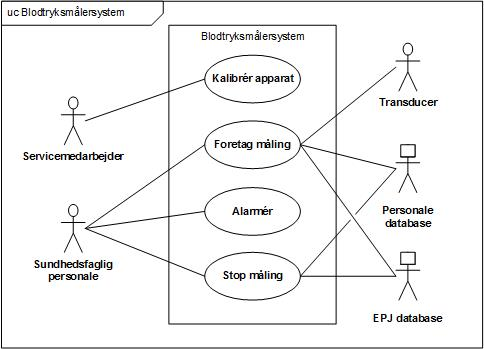
\includegraphics[width =0.7\textwidth , center]{billeder/UseCaseDiagram}
\caption{Use Case diagram. Dette diagram viser aktørernes interaktion med systemet.}
\end{figure}
\section{Aktørbeskrivelse}
Ud fra use case diagrammet ses de seks aktører; \textit{Sundhedsfaglig personale}, \textit{Transducer}, \textit{EKG patient}, \textit{EPJ database}, \textit{Personale database} og \textit{Servicemedarbejder}. Det er disse aktører der interagerer med systemet.
\subsection{Sundhedsfaglig personale}
Det er det sundhedsfaglige personale, der er den aktør, der påsætter måleudstyret på patienten. I dette tilfælde vil patienten være en In vitro maskine. Det sundhedsfaglige personale er desuden den aktør der interagerer med systemet; logger på og foretager en måling. Det sundhedsfaglige personale har dermed adgang til systemet og de viste målinger på brugergrænsefladerne; startskærm og hovedskærm.
\subsection{Transducer}
Transduceren er i projektet den aktør der agere som patienten, denne består af en In vitro maskine tilsluttet katetersystemet, der er påsat en tryktransducer. Katetersystemet leverer et tryk i mmHg videre til tryktransduceren, som omdannet trykket til et digitalt signal. Dette signal sendes videre i hardwaren, som består af en forstærker og et lav pasfilter, som behandler signalet og via NI-DAQ sendes signalet ind i systemet. Derfor er denne aktør kilden til måleresultaterne for systole, diastole og middeltryk.
\subsection{EKG-patient}
EKG patienten er den aktør, som er kilden til EKG-kurven, der ikke haves en rigtig patient, hvorfra både EKG og blodtryk kan indhentes fra. Idet det er fra denne aktør at EKG-kurven findes er det fra denne aktør, pulsen kan bestemmes.\\
Værdierne for denne aktør hentes fra PhysioBank ATM.
\subsection{Servicemedarbejder}
Denne aktør, Servicemedarbejder, er aktøren, der står for at foretage kalibreringen. Dette gør Servicemedarbejderen ved at påsætte systemet til kalibreringssystemet, og indtaster de værdier for tryk (mmHg) og spænding (Volt), som måles ved tre forskellige målepunkter på en vandsøjle, hvorefter en kalibreringsværdi findes af systemet.
\subsection{EPJ database}
EPJ databasen, er databasen, hvori patientdata ligger samt den database hvori måledata bliver gemt. Blodtrykskurvens rådata gemmes som en talliste. For at have nok information om signalet gemmes kalibrerings- og nulpunktsjusteringsværdien for signalet også i EPJ databasen. Denne EPJ database skal simulere den database der fungerer på sygehusene i virkeligheden. Denne database kobler patienterne i denne database sammen med en sundhedsfaglig fra Personale databasen. 
\subsection{Personale database}
Det sundhedsfaglige personales login informationer ligger i Personale databasen. Det er derfor denne database der indeholder informationer om det Sundhedsfaglige personale og dermed de informationer der benyttes til at tilgå systemet.
\section{Use case beskrivelse}
Use case diagrammet viser ligeledes de fire Use cases, der er for systemet: Kalibrér apparat, Foretag måling, Alamér og Stop måling. Disse Use cases er en beskrivelse af, hvad systemet skal kunne og beskriver de interaktioner, der sker mellem aktørerne og systemet.
\\
\subsection{Use case 1: Kalibrér apparat}
Servicemedarbejderen skal i denne Use case foretage en kalibrering. Dette gøres ved at der er tre målepunkter på en væskesøjle, hvor én af disse målepunkter vælges. Fra målepunktet måles spændingen (volt), med et multimeter eller Analog Discovery, og trykket (mmHg) aflæses fra væskesøjlen. Disse indtastes af Servicemedarbejderen ind i systemet igennem brugergrænsefladen; startskærmen. Herefter beregner systemet en kalibrerings værdi. Denne værdi bruges til at omskrive de indlæste værdier, fra DAQ, til en blodtrykskurve i mmHg.
\subsection{Use case 2: Foretag måling}
Denne Use case styrer målingerne af graferne der indhentes. For at dette kan gøres, skal det Sundhedsfaglige personale først logge på systemet. Dette gør denne aktør ved at indtaste sit brugernavn og sin adgangskode på brugergrænsefladen; startskærmen, hvilken repræsenterer en EPJ computer, som virker på hospitalerne. Når den sundhedsfaglige er logget på, henter systemet de tilknyttede patienter, hvorefter det Sundhedsfaglige personale kan vælge den ønskede patient. Når Patienten er blevet valgt startes hovedskærmen, hvilken repræsenterer en blodtryksmålers brugergrænseflade. \\
For at sikre at graferne, der hentes ligger rigtigt på graferne, skal det Sundhedsfaglige personale nulpunktsjustere systemet, sådan at graferne kommer til at ligge rigtigt på akserne. Dette gøres ved at der tages højde for det atmosfæriske tryk.\\
Herefter kan den Sundhedsfaglige starte målingen. Når dette gøres, henter systemet blodtrykssignalet og EKG-signalet. Disse bruges derefter af systemet til at beregne hhv. systole, diastole, middeltryk og puls. Systemet viser graferne kontinuert på hver sin graf og systole, diastole, middeltryk og puls vises som talværdier. Samtidig gemmer systemet automatisk løbende disse data i EPJ databasen. \\
Det vil være muligt for det Sundhedsfaglige personale at slå det digitale filter fra og til. Filteret er pr. default slået til fra start.\\
Det er også muligt for det Sundhedsfaglige personale at justere grænseværdierne for systolen og diastolen, dette gøres for at indstille grænseværdierne individuelt for hver patient.
\subsection{Use case 3: Alarmér}
Alarmen startes af systemet, når en af grænseværdierne for systole eller diastole overskrides. Dette gør at knappen der benyttes til at udsætte alarmen blinker skiftevis mellem at have rød og hvid baggrund og der starter en alarm lyd. Når alarmen er igangsat kan endnu en grænseværdi overskrides, hvis dette sker, sker der umiddelbart ikke noget. Alarmlyden fortsætter fra tidligere, og knappen, til udsættelse af alarmen, fortsætter med at blinke. \\
Det vil her være muligt for det Sundhedsfaglige af udsætte alarmen. Dette gøres ved at trykke på "Udsæt alarm" knappen, hvorefter systemet stopper alarmens lyd i et minut, efter dette minut starter alarmens lyd igen. "Udsæt alarm" knappen fortsætter med at blinke indtil forholdene er normaliseret, altså indtil grænseværdien ikke længere er overskredet.
\subsection{Use case 4: Stop måling}
Det Sundhedsfaglige personale skal også kunne stoppe målingen. Dette gøres ved at det Sundhedsfaglige personale interagere med hovedskærmen. Herefter vil det være muligt for det Sundhedsfaglige personale at logge ud, og et nyt scenarie kan påbegyndes.
\section{Ikke-funktionelle krav beskrivelse}
Ikke funktionelle krav er opsat efter FURPS+ metoden. Kravene er herefter blevet prioriteret efter MoSCoW.
\subsection{FURPS+}
\textbf{Functionality}\\
Funktionalitet er det brugeren ønsker sig. Dette omfatter også sikkerhedsrelaterede behov. Dette er krav til hvad programmet skal kunne af funktionalitet, f.eks. at programmet skal gemme data løbende i en database.\\\\
\textbf{Usability}\\
Hvor effektiv er produktet, set fra forbrugerens side, dette er det aspekt brugervenlighed ser på. Er produktet nemt at bruge. Hvordan bruges produktet; er der nogen brugergrænseflader. Det er herunder kravene til hvilke knapper der skal være på brugergrænsefladerne, og dermed også hvilke brugergrænseflader der skal være.\\\\
\textbf{Reliability}\\
Pålidelighed tager sig af aspekter som, hvor længe er det maksimalt at systemet må være nede. Er der fejl der kan forudses. Hvor præcist kan resultaterne vises. Er produktet let at vedligeholde; kan delene i produktet skiftes let.\\\\
\textbf{Performance}\\
Præstationen for produktet, handler om hvor hurtigt produktet er om at starte op og hvor hurtigt svartiden er. Hvor stor må svartiden maksimalt være. Så det er altså herunder, at det er beskrevet, hvor lang tid der går fra der er trykket på en knap, til at systemet svarer. \\\\
\textbf{S}uportability\\
Produktets support fortæller, om det er muligt at teste på produktet, om det er muligt at udvide produktet, installere og konfigurere produktet. Desuden om produktet er kompatibelt. Det er herunder programmets opbygnings model beskrives\\\\
\textbf{+}\\
Kunden kan have nogle yderligere behov, disse yderligere behov beskrives under +. Hvilke begrænsninger er der ved designet. Er der nogle krav for brugergrænsefladerne. Er der nogle fysiske eller implementerings krav. Er der dele der kan genbruges, herunder hele systemer eller dele af dem. Det er bl.a herunder at kravene til computeren der benyttes beskrives. \cite{furps}\\

\subsection{MoSCoW}
\textbf{Must}\\
De krav der bliver markeret som et must er de krav som produktet skal have. Altså det produktet skal have/indeholde.\\\\
\textbf{Should}\\
De krav der markeres som et should krav, er de krav til produktet der burde være med. Altså er det hvad produktet bør indeholde\\\\
\textbf{Could}\\
Kravene kan også markeres som could. Disse krav er de krav der kunne være gode at have med, men som ikke bliver prioriteret. Så det er kun, hvis man kan nu at få det med, at de skal være der.\\\\
\textbf{Would/Won't}\\
Det er ikke alle krav der skrives, der skal være gældende for produktet, disse krav markeres som would/won't. Det er altså disse krav som man ikke tager med eller de krav som ville være sjove at have med, men ikke har en betydning for produktet, men er en tilføjelse eller udvidelse. Det er disse krav der danner rammen for fremtidigt og videregående arbejde med projektet.
\chapter{Projektbeskrivelse}
\section{Projektgennemførelse}
\subsection{ASE-modellen}
Til udviklingen af dette produkt er der primært benyttet ASE-modellen. Modellen ses herunder. ASE-modellen er en udviklingsmodel, der er udarbejdet af Aarhus Ingeniørhøjskole. Denne model er en mellemvægtig semi-iterativ udviklingsproces, hvilken drives ud fra Use cases. Projektudviklerne fastlægger først en projektformulering, hvorfra en kravspecifikation kan udarbejdes, hvilken indeholder kravene fra kunden. Systemarkitekturen fastlægges ud fra kravspecifikationen, for derefter at designe og implementere de enkelte hardware og software dele hver for sig i iterationer. Til sidst fører dette til en accepttest, hvilken gennemføres, så der opstår een enighed mellem projektudviklerne og kunden.
\begin{figure}[H]
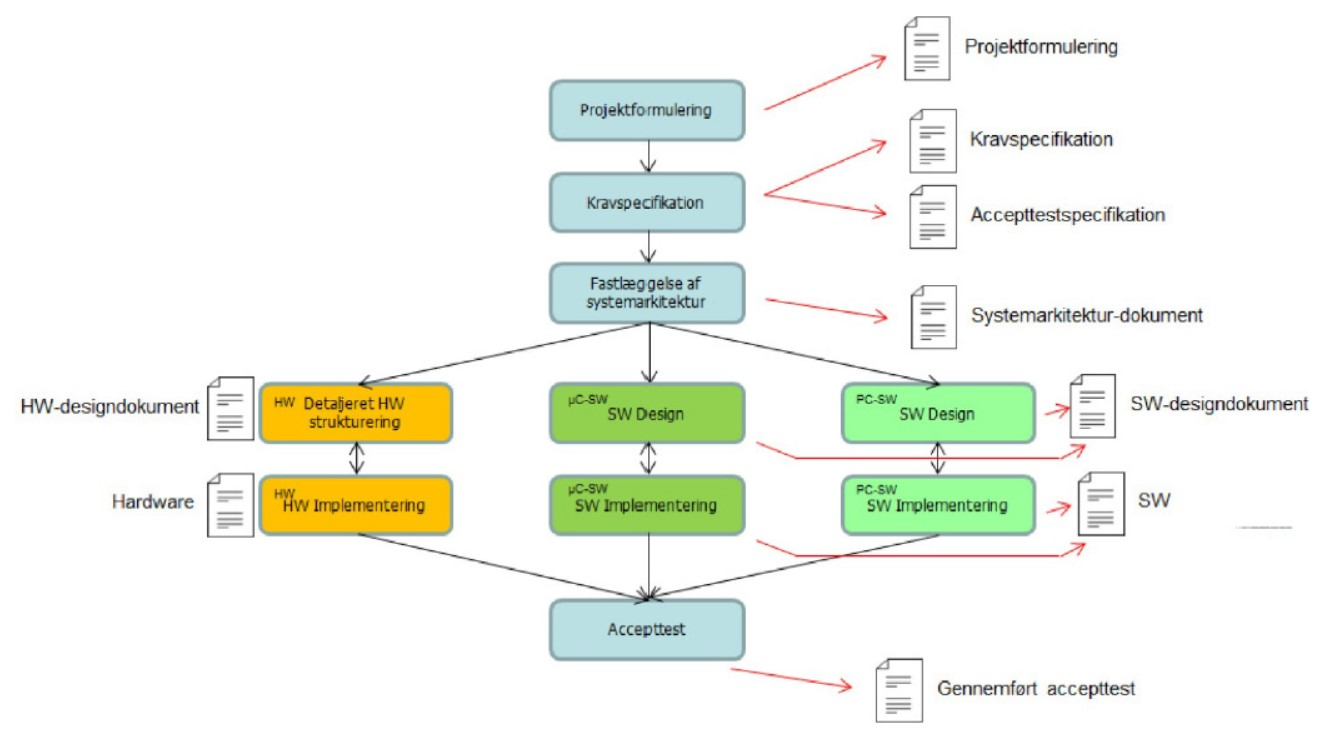
\includegraphics[width =1.0\textwidth , center]{billeder/ASEmodellen}
\caption{ASE-modellen.}
\end{figure} 
Kravspecifikationen bliver specificeret som en række Use cases ud fra problemformuleringen. Use cases benyttes til at beskrive aktørernes interaktion med systemet. Sammen med de ikke-funktionelle krav opnås der med Use casene et overblik over hvilke krav der stilles til systemets funktionalitet. Systemets design bestemmes igennem hardware og software design og implementering, herefter kan en accepttest udarbejdes. Ved udførelsen af accepttesten tjekkes det at kravene er opnået.
\subsection{V-modellen}
V-modellen er en faseopdelt udviklingsmodel. Denne model beskriver udviklingsfaserne og testfaserne i et projekt sideløbende. V-modellem er blevet benyttet sideløbende med ASE-modellen. Specifikationen af test foregår parallelt med udviklingen af selve systemet i V-modellen. Fordelen ved denne model er at testene sker på forskellige niveauer, hvilket sikre at udviklede delsystemer virker som ønsket. Det vigtige her er at en fase er færdiggjort, inden den næste fase påbegyndes. 
\begin{figure}[H]
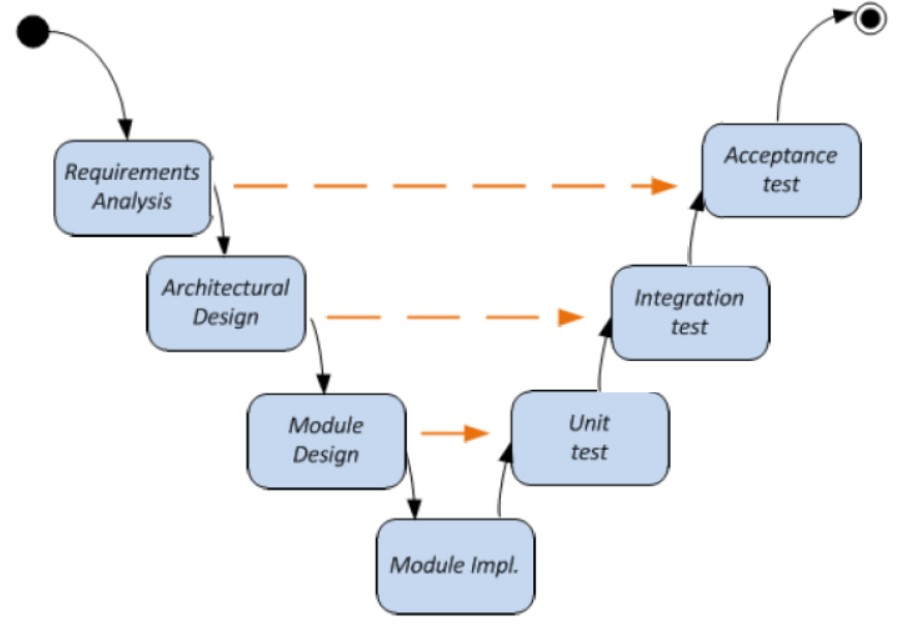
\includegraphics[width =0.7\textwidth , center]{billeder/Vmodel}
\caption{V-modellen.}
\end{figure} 
Ud fra modellen ses det at den første fase er udviklingen af kravspecifikationen. Her udarbejdes der en tilhørende accepttest, denne test gør det muligt at tjekke om systemet til sidst lever op til de opstillede krav. Den næste fase er herefter systemarkitektur, her udvikles den tilhørende test, denne test undersøger integrationen mellem de implementerede moduler. De sidste to fase af udviklingsfasen er design og implementering af systemets enkelte moduler, her udføres enhedstesten løbende af de implementerede moduler.
\subsection{Vandfaldsmodellen}
Vandfaldsmodellen er en model der bruges til udvikling af software og hardware, hvor software- og hardwareudviklingen betragtes som værende konstant nedad løbende. Her kan udviklingen af et modul i en ny fase først påbegyndes når den foranliggende fase er afsluttet. Denne model et i projektet benyttet til udviklingen af software- og hardwarearkitekturen. 
\begin{figure}[H]
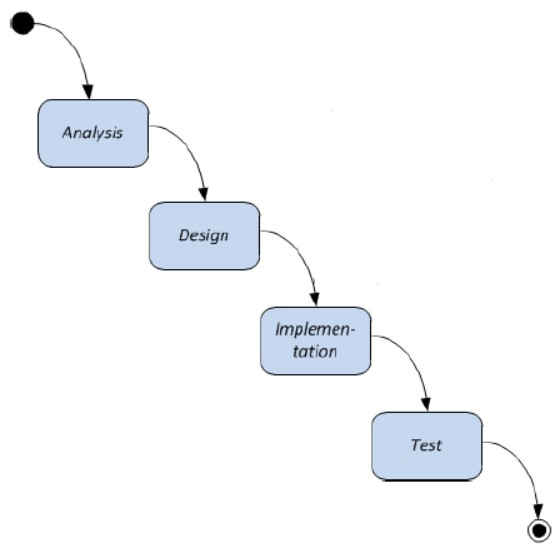
\includegraphics[width =0.5\textwidth , center]{billeder/Vandfald}
\caption{Vandfalds modellen.}
\end{figure} 
Disse tre modeller; ASE-modellen, V-modellen og vandfalds-modellen arbejder alle i en kronologisk logisk rækkefølge. Modellerne er benyttet i et omfang, hvor de har kunnet supplere hinanden. ASE-modellen giver det store overblik, mens V-modellen sikre udarbejdelsen af de nødvendige tests. Vandfalds-modellen er den proces, hvilken der er arbejdet ud fra i alle projektets facetter.   
\subsection{Projektstyring}
\subsubsection{Arbejdsfordeling}
Som nævnt tidligere valgte man fra projektets start at opdele gruppen i to hold, henholdsvis et softwarehold og et hardwarehold.
\subsubsection{Ændringer i projektstyring}
Under projektforløbet valgte vi at ændre denne rollefordeling, idet den generelle arbejdsfordeling samt arbejdsindsats i gruppen ikke fungerede optimalt. Vi valgte, at kun et gruppemedlem skulle varetage rollen som projektleder og procesleder, men at opgaver herunder kunne uddelegeres hvis nødvendigt. Denne leder blev i fællesskab valgt og baggrunden for dette valg var, at vi ønskede en leder som både havde viden og indflydelse på hardware og software, samt kunne gribe ind hvis gruppearbejdet og deltagernes indsat ikke opfyldte den forventningsafstemning, som står skrevet i vores samarbejdskontrakt. 
\subsubsection{Scrum}
Det blev i øvrigt besluttet at benytte SCRUM som hjælp til styring af projektet. Der blev udnævnt en tovholder som skulle holde møder i løbet projektets udarbejdelse samt styre opgaverne. Man valgte at bruge Pivotal Tracker \cite{tracker}  til at styre og prioritere opgaver. Der var en overordnet tidsplan fra start, denne tidsplan består af en række deadlines – den kan findes i dokumentationen.
\subsubsection{GitHub}
Det blev besluttet at benytte GitHub til deling af informationer og dokumentation i forbindelse med udarbejdelse af rapporten. Det blev vurderet at det var vigtigt at der var en central informationsudveksling så begge grupper kunne følge med i hvor langt de var i de forskellige processer. 
\subsubsection{Iterativ udviklingsproces}
Udviklingsprocessen på både software- og hardware-holdet blev meget iterativ, det betød at der var mange forskellige versioner af både hardware og software. Man valgte denne metode da store dele af projektet var et teknologistudie, så det var nødvendigt at lave mange iterationer løbende. Desuden var det vigtigt at de to hold kunne omstille sig hurtigt, og drage ny viden til nytte uden at skulle igennem en langsommelig design proces på ny.
\section{Metode}
\cite{SysML} For at beskrive den overordnede systemarkitektur og det detaljerede design for produktet, er der blevet benyttet SysML og UML. SysML er et grafisk modelleringssprog, hvilket kan hjælpe til at forstå og udvikle selv komplekse systemer. SysML udspringer af UML, dog benyttes SysML i højere grad ved systemer, der både indeholder software og hardware, end UML. UML benyttes til at beskrive softwaresystemets struktur og forløb. \cite{uml}
\\
\\
SysML’s struktur-, funktionalitets og adfærdsdiagrammer er i projektet blevet benyttet til at specificere og dokumentere systemet og dets komponenter. Der anvendes to strukturdiagrammer; block definition diagram (BDD) og internal block definition diagram (IBD) for at vise systemstrukturen. Systemarkitekturen bliver delt op i blokke. BDD'et bruges til at vise forholdet mellem de forskellige blokke, deres komposition og forholdet mellem logiske- og fysiske enheder i systemet. IBD'et benyttes til at vise den forbindelse der er imellem de forskellige blokke der ses ud fra BDD'et. Dermed ses den vej signalet går igennem de forskellige enheder og hvordan disse enheder er koblet sammen.\\
\\ 
For at kunne beskrive produktets funktionalitet er der blevet udarbejdet et Use case diagram. Dette diagram beskriver, hvordan systemet interagerer med de udefrakommende enheder (f.eks. aktører) for at løse et antal af opsatte opgaver. Disse opgaver er beskrevet i forskellige Use cases. \\
Domænemodellen beskriver det overordnede systemdomæne. Systemdomænet beskrives ud fra de konceptuelle klasser, hvilke findes ud fra Use cases. Domænemodellen definere de klasser, der skal være i softwaren og de interaktioner der er imellem disse, dette gøres med klassediagrammer og adfærdsdiagrammer.\\
Et af adfærdsdiagrammerne er et sekvensdiagram, denne viser de handlinger der er mellem systemets dele (parts), hvilke er delt op i sekvenser.\\
For at beskrive overgangen fra de beskrevne Use cases til software, er applikationsmodellen benyttet. Applikationsmodellen tager udgangspunkt i Use cases og domænemodellen, hvor Use cases bruges til at identificere, hvad systemet skal kunne og hvordan det skal løses. \\
\\
En applikationsmodel med kontrolklasser, domæneklasser og boundaryklasser kan opbygges. Kontrolklasserne har funktionen at beskrive hvordan data behandles mellem domæne- og boundaryklasserne. Domæneklasserne indeholder funktionaliteten som det pågældende softwaremodul benytter, det er herfra klasserne, der skal bruges i softwaren identificeres. Boundaryklasserne har den funktion at beskrive hvordan systemet kommunikerer med omverdenen og omvendt. Ved at benytte applikationsmodellen til design af softwarens opbygning, gøres det lettere at udvikle et produkt med lav kobling samt høj samhørighed. \\
\\
Systemets softwarestruktur og forløb beskrives ved at benytte UML klassediagrammer. Klassediagrammet viser den struktur der er mellem et objektorienteret systemklasse, og kan derfor bruges til at definere relationen mellem de forskellige klasser. Derfor dannes der et hurtigt overblik over sammenhængen i systemet ved at benytte klassediagrammet.  
\section{Specifikation og analyse}
I det følgende afsnit beskrives de overvejelser der er gjort i projektet i forbindelse med specifikation og analyse af henholdsvis hardware og software delen. Gennem afsnittet startes der med at kigge på hvilke specifikationer der er valgt, analysen og grunden til dette. Afsnittet er inddelt i at først kigge på specifikations og analyse arbejdet angående det lavpasfilteret og operationsforstærkerne. Derefter vil der blive beskrevet specifikations og analyse arbejdet angående det digitale filter, udregning af blodtryksværdi og præsenter data på en pæn måde på et brugergrænseflade.
\subsection{Hardware}
En af de krav der var til Hardwaren givet fra projektets vejledning var, at der skulle designes et lavpas filter med en cut-off frekvens på 50 Hz. Et andet krav var at filteret skal kunne dæmpe med 20db pr. dekade ved 500 Hz. Der bliver desuden opgivet at kondensatoren C2 skulle have en værdi på 680 nF. \\
Der var også opgivet krav til filteret at det skulle være et anden ordens butterworth sallen key filter. Herved er der valgt. \\
Ud fra krav omkring filteret og værdien af kondensatoren, er der opstillet overføringsfunktionen for Salle-Key anden ordens filteret. Overføringsfunktionen er udformet ud fra vejledningen for det faglige indhold, som indeholdte de krav der var opgivet til projektet, fra skolen.
\begin{align}
\dfrac{V_{out}(s)}{V_{in}(s)}=\dfrac{\dfrac{1}{R1\cdot R2\cdot C1\cdot C2}}{s^2+\dfrac{R1+R2}{R1\cdot R2\cdot C2}\cdot s+\dfrac{1}{R1\cdot R2\cdot C1\cdot C2}}
\end{align}
Analysen af filteret er lavet, ved at omskrive overføringsformlen til en standard formel for anden ordens filtre. I standard formlen for anden ordens filtre, er der isoleret cut-off frekvensen, og opstillet en ligning for denne. \\
Igennem arbejdet med analysen af filteret, blev der efter flere iterationer, fundet ud af at værdien for kondensatoren C1, skulle være det halve af C2. Værdien for C1 kunne udregnes til 340nf. \\
Da der nu er specificeret værdier for begge kondensator og en ligning for cut-off frekvensen, som også er specificeret til 50 Hz, er de to modstande R1 og R2 udregnet. 
\begin{figure}[H]
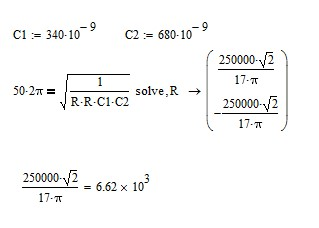
\includegraphics[width =0.3\textwidth , center]{billeder/mathcad2}
\caption{\textbf{Beregning fra Mathcad}}
\end{figure}
Alle komponent værdier er specificeret for vores anden ordens butterworth sallen-key filteret. For at sikre sig at specifikationerne er sat til de rigtige værdier, er der lavet en analyse i matlab ved at lave et bodeplot over amplituden. På bodeplottet kigges derefter om grafen falder ved 50 Hz, og om der er faldet 20 db pr. dekade ved 500 Hz. På bodeplottet herunder ses det at grafen er dæmpet 3dB ved 50 Hz, hvorfra det kan konkluderes at specifikationerne for filteret er rigtige. Der kan også aflæse fra grafen at filteret er faldet 20dB pr dekade, dette ses ved at fra cut-off frekvensen på 50 Hz, går der en dekade før den er faldet til en amplitude 40 db, som svare til en frekvens på 500Hz. 
\begin{figure}[H]
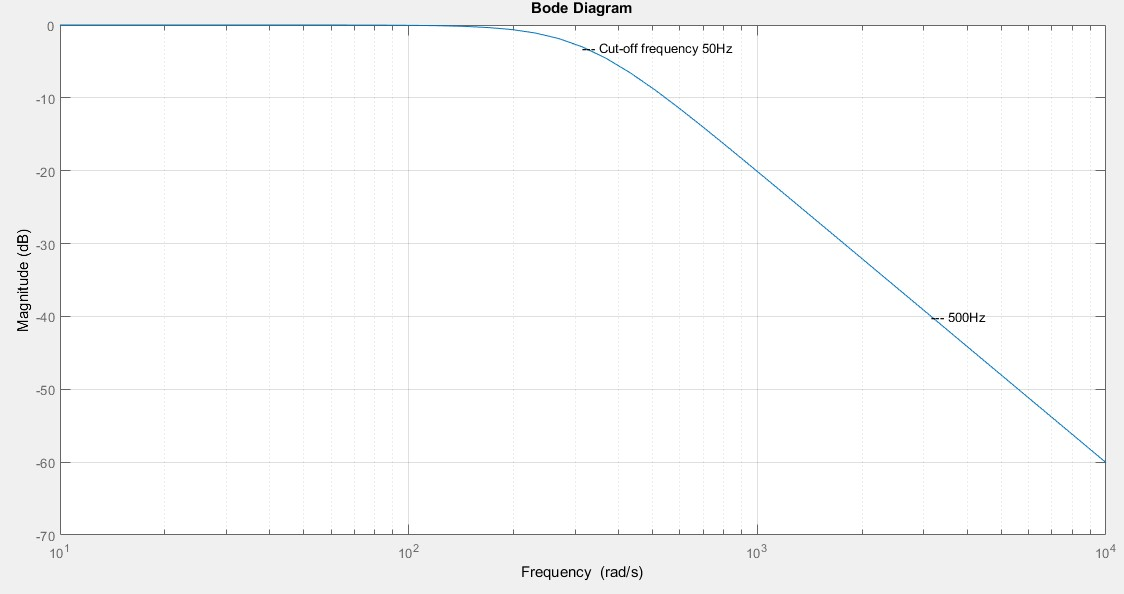
\includegraphics[width =0.6\textwidth , center]{billeder/bodeplot}
\caption{\textbf{Bodeplot}}
\end{figure}
Operationsforstærkeren For at kunne dimensionere operationsforstærkeren tilfredsstillende, kiggede man på de allerede forelagte krav samt hardwaredele der var til stede. Det elektriske signal fra tryktransduceren(TruWave\texttrademark) som skulle sendes i vores dataopsamlingsmodul (NI-DAQ6009), skulle således forstærkes i tilstrækkelig grad. Dette giver større præcision i vores målesignaler og mindre fejlmargin. Den maksimale spænding DAQ’en kunne tage imod er +/- 10V, det vil sige der ikke måtte forstærkes mere op en +/- 10V. Man valgte at benytte en INA114 efter anbefaling fra medstuderende og vejleder. Til forstærkeren valgte man to 9V-batterier som spændingsforsyning, dette ville give os teoretisk maksimal forstærkning på +/- 9V, da vi valgte at bygge spændingsforsyning op så den ville levere 18V peak-to-peak. Man sikrede sig ved hjælp af udregninger at båndbredden og den gain der kunne leveres var tilstrækkelig i INA114-forstærkeren. Ligeledes udregnede man størrelsen på den modstand der regulerer gain, det blev besluttet at benytte et potentiometer i stedet for en fast modstand for at imødekomme evt. udsving i forbindelse med opbygning på fumlebræt samt \%-tolerance i komponenter.
\subsection{Software}
I projektvejledningen var der opstillet krav omkring at softwaren skulle implementere digitalt filter, skulle kunne vise data kontinuert, kunne kalibrere og foretage en nulpunktsjustering, gemme data i enten en tekstfil eller database og det digitale filter skal kunne slås til og fra. \\
Der er implementeret et moving avearge filter, som tager gennemsnittet af blodtrykstallene og sender videre. Efter snak med vejledere er der valgt et moving average filter. Fordelen ved dette filter er at det udglatter hver enkelt værdi for blodtrykket, i stedet for at udglatte få områder af blodtrykssignalet. Filteret bliver herefter ganget på alle værdierne for blodtrykket. Der er valgt dette filter fordi det kan bruges på et kontinuert signal, da det bare udregner gennemsnittet på det den har fået ind, og udregner et nyt gennemsnit ud for hvert tal. \\\\
Kravet om at kunne kalibrere er blevet specificeret ved at oprette en kalibreringskoefficient. Denne kalibreringskoefficient er fundet ved at benytte en væskesøjle, som levere et tryk på 50mmHg på et punkt, hvor spændingen i punktet blev målt til 1V. Dette gav en kalibrering koefficienten til 50. Denne kalibrerings koefficient er implementeret i software koden i en appconfig fil, som er en xml fil. Dette er valgt, fordi der ikke kalibreres hver gang, er der en default kalibreringsværdi som koden kalibrerer efter. Herved kan sygeplejerskerne springe kalibrering over, og gå direkte til måling efter at have logget ind. Der skal kalibreres en gang om året, herved er kalibrering indsat på StartGUI, hvor værdien for tryk og spænding kan indtastes, herefter udregner programmet kalibreringskoefficienten ved at divider disse to, og gemme dem som en lokal variable. \\\\
Kravet om at kunne vise en måling kontinuert er løst ved at bruge Observer mønstret, hvor der er tilknyttet et subject til, som hele tiden giver besked om der er sket ændringer.  Observer mønsteret er valgt, da det giver mulighed for at sende data imellem to klasser, hver gang der bliver indlæst nye tal af DAQ’en. Observer mønsteret er også valgt til at sende analyseret data fra logiklaget til præsentationslaget på brugergrænsefladen. For at vise data kontinuert er der lavet en kø og en update metode, som hele tiden opdater grafen op på brugergrænsefladen. Køen gør at der puttes en masse tal ind i en række, og præsenter det nyeste tal i køen først, på brugergrænsefladen. \\\\
Efter analyse af dette mønstre er der vurderet at opbygge det efter push princippet, så hver gang der bliver indlæst et tal fra DAQ’en bliver dette tal via subjectklassen sendt videre fra daqklassen til logiklaget. Dette sørger for at data bliver sendt op igennem programmets trelags struktur. \\\\
Der er specificeret to databaser: EPJ database og Personale database. Til at gemme data, herunder blodtrykssignalets rådata er EPJ databasen blevet benyttet. I denne database ligger samtlige patient oplysninger. For at kunne koble de to databaser sammen er hver patient er koblet til en sundhedsfaglig. Det sundhedsfaglige personales oplysninger ligger i Personale databasen. Der er valgt at det skal være databaser, i stedet for en fil, da der skal kunne ligges data i og hentes data fra databasen fra forskellige computere og servere. Informationerne om patienten er vigtige, for at kunne diagnosticere nuværende anormaliteter og grunden dertil. Ved at sammenligne de nye målinger med tidligere vil disse anormaliteter nemlig kunne bestemmes. Patientens navn og cpr bliver vist på Hovedskærmen, for at være sikker på at det er den rigtig patient der er fat i. \\\\
Nulpunktsjustering er et krav der et opgivet i projektvejledningen. Efter snak med vejleder er der specificeret at nulpunktsjustering skal ske efter at signalet er indlæst af DAQ’en. Det er blevet analyseret frem til at der skal nulpunktsjusteres for det atmosfæriske tryk igennem transduceren. Efter videre analyse er det kommet frem til at det atmosfæriske tryk er en tilnærmelsesvis ret linje. Det atmosfæriske tryk måles manuelt ved at åbne for transduceren, så det blot er det atmosfæriske tryk der måles på. Igennem systemet måles denne værdi. Denne værdi indskrives på hovedskærmen, hvorefter systemet tilpasser for denne værdi, når der trykkes på "Nulpunktsjustering". Det er specificeret at nulpunktsjusteringsværdien lægges til samtlige blodtryksværdier. Inden signalet bliver vist på grafen, bliver kalibreringskoefficienten ganget på samtlige blodtryksværdier. Dette er valgt for at undgå en større ændringer af blodtrykssignalet, når det er vist på grafen.  

	\section{Arkitektur}
	\subsection{Hardware}
	kort indledning
	Hardware beskrivelse
	Signalets vej
	BDD/IBD indsættes
\subsection{Software}
Systemets softwarearkitektur beskrives på baggrund systembeskrivelsen og kravspecifikationen. Ud fra relevante diagrammer og modeller kan software beskrives hvorfra arkitekturen for softwaren opnås. Samtlige diagrammer og modeller kan findes i Projektdokumentationen under Arkitektur og design.
\subsubsection{Problemidentifikation}
Først skulle det identificeres hvad produktet skulle bruges til og hvordan det skulle virke. Her blev der i først omgang ud arbejdet en idé til at produktet skulle benyttes ved blodtryksmåling på diabetes patienter. Dette førte til at der blev lavet en startskærm, hvorfra det kunne vælges, hvor målingen skulle foretages, sådan at data efterfølgende kunne analyseres. Dette skulle føre til en diagnosticering af hvor slem diabetes patienten havde og dermed hvor lavt blodtrykket er ude i underekstremiteterne. Denne hypotese er dog ikke blevet afklaret, idet idéen blev kasseret. Det blev nemlig klargjort at foretage en invasiv blodtryksmåling i underekstremiteterne, på en diabetes patient, hvor dette ikke vides præcist hvor lavt blodtrykket er i underekstremiteterne, ville være en rigtig dårlig idé. Dette er den, fordi en direkte invasiv blodtryksmåling foregår ved at systemet påsættes patienten via en arteriekanyle. Da en diabetes patient har lavere blodtryk i underekstremiteterne og dermed dårligere blodstrømning, vil det være en dårlig idé at påsætte en arteriekanyle, dette vil kunne resultere i en infektion. En ny idé blev derfor udarbejdet. Her skal produktet ligne en blodtryksmåler, som ligner dem der findes på hospitalerne og sygehusene. Derfor blev et møde med anæstesi sygeplejerske Charlotte Høj fra Herning sygehus afholdt. Her blev et blodtryksmålingsscenarie vist. På EPJ-systemet (EPJ-computer) skulle man først logge på, hvor patienten på hvem målingen skulle foretages kunne vælges. Herefter kunne blodtryksmålingen foretages på patienten. Denne idé blev dermed idéen til projektet.\\\\
Ud fra denne idé kunne Use cases udarbejdes, disse er beskrevet under Krav, hvor hovedscenariet for brugen af blodtryksmåleren beskrives.
\subsubsection{Domænemodel} 
Ud fra disse Use cases kunne de klasser som systemet skulle bestå af identificeres. Disse klasser identificeres ved at bestemme de konceptuelle klasser, som indeholder den information som systemet skal holde styr på. De konceptuelle klasser indføres i domænemodellen som klasser. Det er i domænemodellen hvor problemet i forhold til hvad der skal holdes styr på i softwaren kan bestemmes. 
\begin{figure}[H]
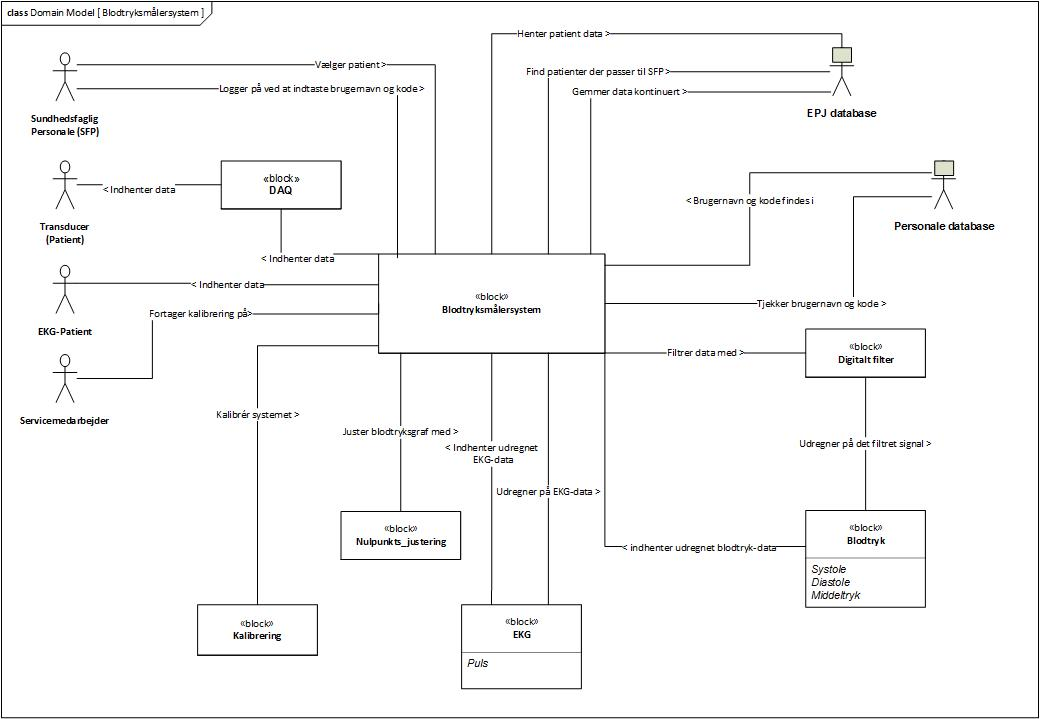
\includegraphics[width =1.0\textwidth , center]{billeder/DM}
\caption{\textbf{Domænemodel for blodtryksmålersystemet.}}
\end{figure}
Ud fra denne model ses det sundhedsfaglige personales interaktion med systemet, samt hvilke handlinger der igangsættes af denne interaktion. Det sundhedsfaglige personale udfører en handling, der medfører, at en række processer starter i systemet. Disse processer sørger for
at hente data fra transduceren og EKG patient, samt sørger for at starte beregningen af værdierne for puls,
systole, diastole og middeltryk. Efter beregningerne viser systemet disse værdier på brugergrænsefladen, samt sørger for at disse data bliver gemt i EPJ database. 
\subsubsection{Klasseidentifikation}
Ud fra domænemodellen kan softwareklasserne altså identificeres. Dette fører til at en applikationsmodel kan opstilles. Applikationsmodellen bruges til at bestemme de interagerende klasser i blodtryksmålesystemet og hvordan disse klasser kan tale sammen. Det er altså også ud fra applikationsmodellen at det kan bestemmes, hvilke klasser der skal ligge i de forskellige lag i trelagsmodellen, da klasserne i applikationsmodellen kan være af typen; domain, boundary og control.\\\\ Controlklasserne (kontrolklasserne) er de klasser er udfører Use casene ved at interagere med domain- og boundary klasserne. Boundaryklasserne (grænseklasserne) er de klasser der repræsenterer aktørerne fra Use Casene og disse aktøres grænseflader. Domainklasserne (domæneklasserne) er de klasser hvori data bliver behandlet og bearbejdet. Domæneklasserne er de klasser der skal ligge i logiklaget. Præsentationslaget og datalaget indeholder begge boundaryklasserne, det skal derfor identificeres hvilke indeholder data og hvilke klasser hvorfra interaktionerne startes.
\subsubsection{Metodeidentifikation}
Ud fra klasserne identificeret af domænemodellen og applikationsmodellen, kan sekvensdiagrammer laves. Sekvensdiagrammerne er interaktionsdiagrammer og viser derfor hvordan processerne forløber i forhold til hinanden. Der laves et sekvensdiagram for hver Use case. Ud fra sekvensdiagrammerne kan det altså ses hvornår og hvordan de forskellige processer forløber i systemet og interagerer med hinanden. Softwaremetoderne kan derfor identificeres ud fra sekvensdiagrammerne. Ud fra sekvensdiagrammerne kan et klassediagram laves. Dette diagram viser hver metode og attribut i hver klasse.
\section{Design, implementering og test}
\subsection{Software}
Ud fra arkitekturen kan designet af softwaren bestemmes. Det bestemmes hvilke mønstre der skal benyttes og hvordan data skal transporteres igennem koden.
\subsubsection{Observer mønsteret}
Observer/subject mønstreret bruges til at sende data op kontinueret og på en fornuftig måde. Subject har en metode til at koble en observer til, og en anden metode til at fjerne observeren. Der er en tredje metode i subject, kaldet notify. Notify sørger for at give besked til den tilknyttet observer om opdatering. En observer er interesseret i at kende til ændringer i det subject den er tilknyttet. Beskeden om ændring kommer fra subjectet, der er tilknyttet observeren. \\
\\
I dette projekt er der valgt at bruge observer/subject mønstreret til at sende data fra datalag til logiklaget. Mønstreret er også brugt til at sende data videre fra logiklaget til præsentationslaget. Yderligere beskrivelse findes i projektdokumentationen under kapitlet Arkitektur og design under afsnittet Software design. 
\subsubsection{PUSH/PULL}
PUSH/PULL er to forskellige måde at implementere Observer mønsteret på. Her bliver data enten skubbet eller trukket op. PUSH betyder at skubbe, og betyder at data bliver skubbet op, når der sker en ændring, uden der skal gives besked om at hente data. PULL trækker data op imellem lagene. I PULL gives der besked til et lag om en ændring. Herefter skal laget, der ønsker at kende til ændringen bede om ændringen, før det sendes op.\\
\\
I dette projekt er det valgt at benytte PUSH til at sende data imellem lagene. Idet det er interessant at få data op til brugergrænsefalden hele tiden når der ny data fra DAQ’en. Yderligere beskrivelse findes i projektdokumentationen under kapitlet Arkitektur og design under afsnittet Software design. 
\subsubsection{Queue}
For at sikre at data bliver sendt op i den rigtige rækkefølge og på en kontrolleret måde, er der i dette projekt valgt at benytte en kø. Til dette er der benyttet en indbygget funktion i Visual Studio, Queue class. Herunder ligger der to metoder, som kan bruges til at sende objekter af tal ind i den ene ende af køen og efter at køen er blevet fyldt op, er der en funktion til at fjerne det første objekt fra den anden ende af køen. Dette sørger for at der hele tiden er et flow i køen når der sendes data ind i denne. \\
\\
En yderligere beskrivelse af hvordan Queue klassen benyttes i koden og hvordan denne er opbygget er beskrevet i dokumentationen under Arkitektur og design under afsnittet Implementering.
\subsubsection{Trelagsmodel}
Trelagsmodellen er en software model, til at inddele sin software i tre lag, præsentationslaget, logiklaget og datalaget. Hver lag har sit eget ansvar og funktionalitet. Præsentationslaget kan kun tilgå logiklaget, og må kun vise data på brugergrænseflade eller indlæse data fra brugergrænsefladen. Logiklaget må tilgå både datalaget og præsentationslaget. Logik er det midterste lag, og står for behandling af data fra præsentationslaget og datalaget. Datalaget er det nederste lag og sørge for at sende data fra et måle apparat op til logiklaget. Datalaget står også for at gemme data i en fil eller en database.\\
\\ 
I dette projekt er koden opdelt efter trelagsmodellen, ved at have et præsentationslag med to brugergrænsefalder, et logiklag med algoritmer til udregning af blodtryk, og et datalag der hente data fra DAQ’en og gemmer dem i en database.  Yderligere beskrivelse og model over trelagsmodellens inddeling af software koden findes i projektdokumentationen under kapitlet Arkitektur og design under afsnittet Software design. 
\subsubsection{Unittest}
Det er blevet besluttet at lave unittest på softwaren. Unit-test forstås ved at der testes på hvert enkelt komponent i koden, i objektorienteret kode vil det sige metoderne. Man sikrer sig at metoderne returnerer det forventede. En unit test bør foregå løbende lige så frit som koden bliver udviklet, så kan man fokusere på de del-elementer som ikke virker efter hensigten. \\
\\
I dette projekt blev der valgt at lave unit-test efter sidste iteration af koden, da de sidste versioner af softwaren ændrede sig meget, så alle unit-tests skulle laves forfra. Grundlaget for mange metoder ændrede sig løbende. Disse unit-tests blev lavet i koden ved at sætte breakpoints og følge metoden til ende og evaluere på hvorvidt metoden opførte sig efter hensigten. Unit-tests er blevet foretaget i koden, hvor der er skrevet kommentarer i koden til de metoder der er blevet testet.
\section{Resultater og diskussion}
Igennem integrationstesten og accepttesten er der opnået resultater for projektet. Igennem accepttesten er der opstillet krav til hvordan blodtryksmålesystemet skal opføre sig i forhold til Use cases, og hvordan dette kommer til udtryk visuelt. Resultaterne for projektet er visuelle resultater af accepttesten, og ses i dette afsnit som screendumps. \\\\
I accepttesten er det første step for accepttest af Use case 1, er at vælge en værdi på vandsøjlen og kalibrer efter den. Herved skal den aflæste spænding og trykket i vandsøjlen indtastes. Når programmet starter, vises start skærmen neden for.
\begin{figure}[H]
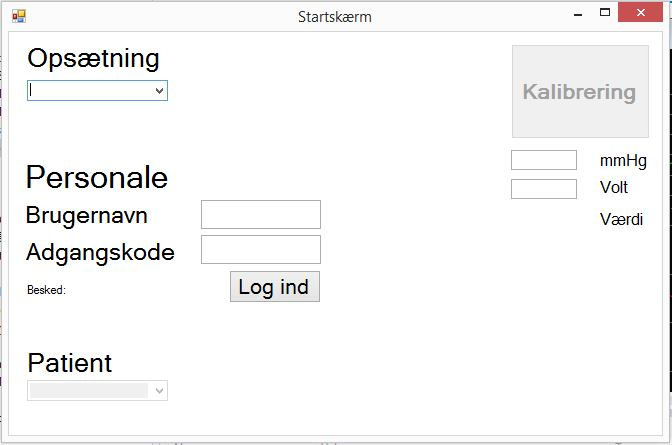
\includegraphics[width =0.4\textwidth , center]{billeder/ITstartGUI}
\caption{\textbf{Startskærm uden indtastede login oplysninger.}}
\end{figure}
Der kan ses på figuren neden for at det er muligt at kalibrer på hovedskærmen, og at blodtryksmålersystemet selv udregner en kalibreringsværdi ud fra de indtastede oplysninger. Kalibreringsværdien udregnes først, når der er trykket på kalibreringsknappen. 
\begin{figure}[H]
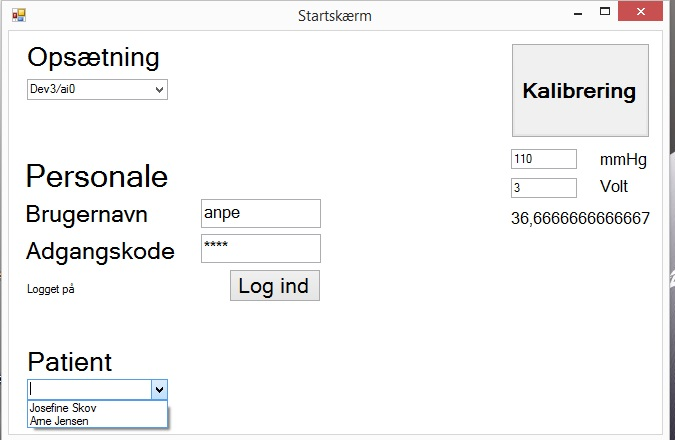
\includegraphics[width =0.4\textwidth , center]{billeder/ITstartGUIlogKali}
\caption{\textbf{Startskærm med login oplysninger og kalibreringsværdi.}}
\end{figure}
Næste step i accepttesten er for Use case 2, er at indtaste brugernavnet "anpe" og koden "1234". Derefter trykkes der på login og vælge patient i patient dropdown. Inden dette er sket er der valgt den port, som DAQ’en er tilkoblet computeren i, og der er logget ind på VPN. På figuren oven for, kan der ses at der er indskrevet brugernavn og adgangskode for anpe, og der vises hvilke patienter anpe kan tilgå i Patient-dropdown. Efter at have valgt en patient i patient dropdown, kommer hovedskærmen frem. Her skal der trykkes på tænd-knappen, og derefter bliver grafen for blodtrykket vist, samt værdierne for systolen, diastolen, middeltrykket og pulsen. Det ses på figuren neden for at blodtrykket bliver vidst med filteret på, og der vises en puls værdi på 69, samt en systole på 125, en diastole på 83 og et middeltryk på 96.
\begin{figure}[H]
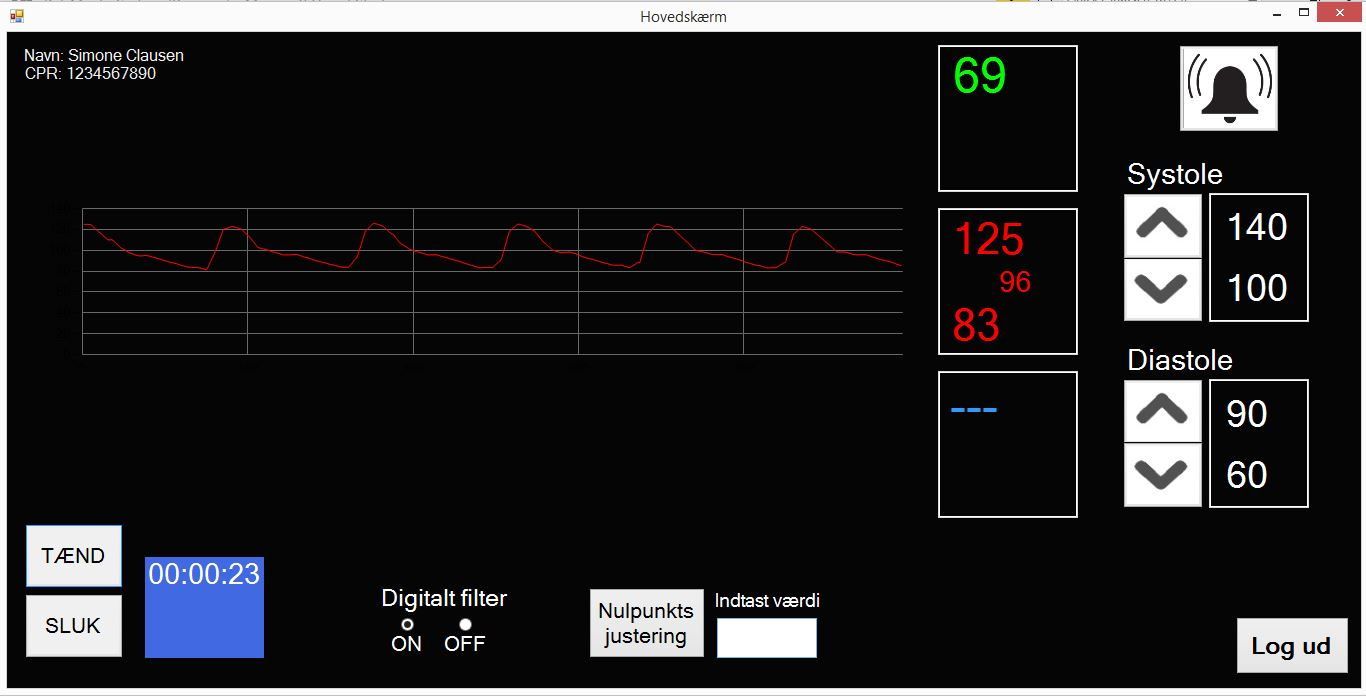
\includegraphics[width =0.6\textwidth , center]{billeder/IThovedGUIkorer}
\caption{\textbf{Blodtryksmåling med det digitale slået til.}}
\end{figure}
Blodtryksmålersystemet skal også kunne angive hvis brugernavnet/adgangskoden ikke findes i databasen. Herved er der i accepttesten for Use case 2, indtastet brugernavnet efgh og koden 1234. Ingen af disse findes i personale databasen, og kan herved ikke bruges til at logge ind med. Som det ses på figuren neden for, er det heller ikke muligt at logge ind, og programmet giver besked om, at brugernavn og/ eller kode er indtastet forkert.
\begin{figure}[H]
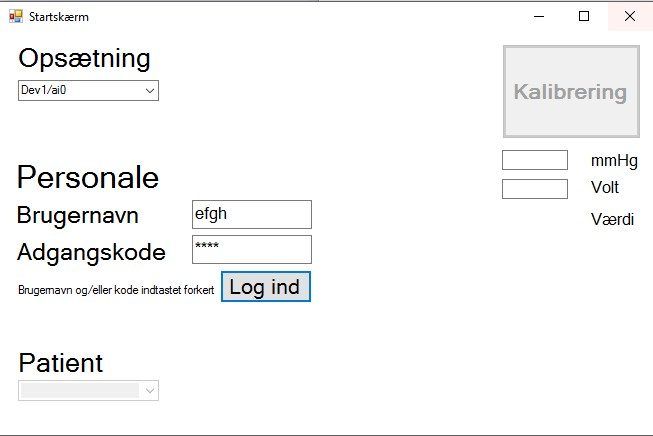
\includegraphics[width =0.4\textwidth , center]{billeder/ITstartGUIforkert}
\caption{\textbf{Brugerneavn/kode er indtastet forkert.}}
\end{figure}
I blodtryksmålesystemet skal det være muligt at kunne slå filteret til og fra, dette bliver testet i accepttesten ved at klikke i radiobutton for digitalt filter off. På figuren neden for, ses at det blodtrykssignalet er forvrænget, da der er kommet mere støj på signalet, herved kan det konkluderes at filteret virker. 
\begin{figure}[H]
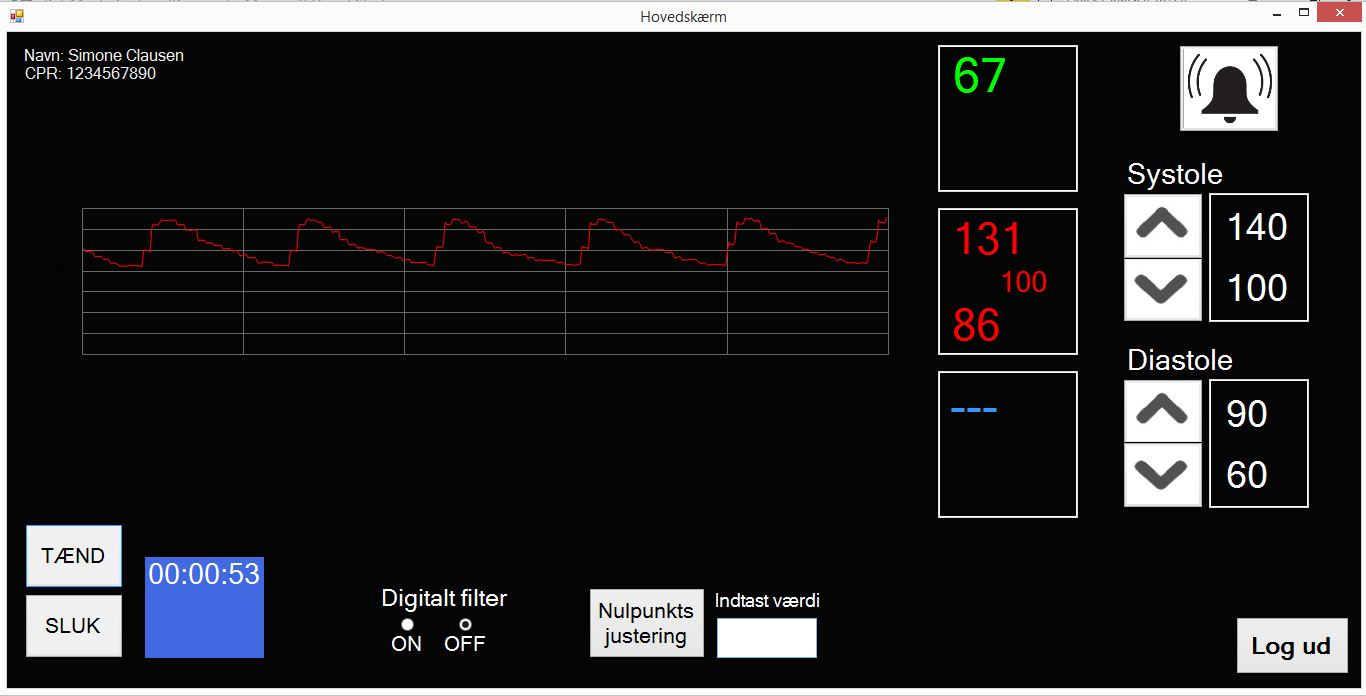
\includegraphics[width =0.6\textwidth , center]{billeder/IThovedGUIkorerufiltreret}
\caption{\textbf{Blodtrykssiganelet uden digitalt filter.}}
\end{figure}
I accepttesten skal blodtryksmålersystemet kunne melde alarm når grænseværdierne overskrides, og grænseværdierne skal kunne ændres på hovedskærmen. På figuren neden for, ses det at grænseværdierne for systolen op og ned, er ændret til 129/89, hvor de før var sat til normal værdierne for systolen, 140/100. Blodtrykssignalet har en systoleværdi på 132, hvilket er over den nye grænseværdi på 129, og derved går alarmen i gang, som det ses med den røde alarm klokke øverst i højre hjørne af hovedskærmen. 
\begin{figure}[H]
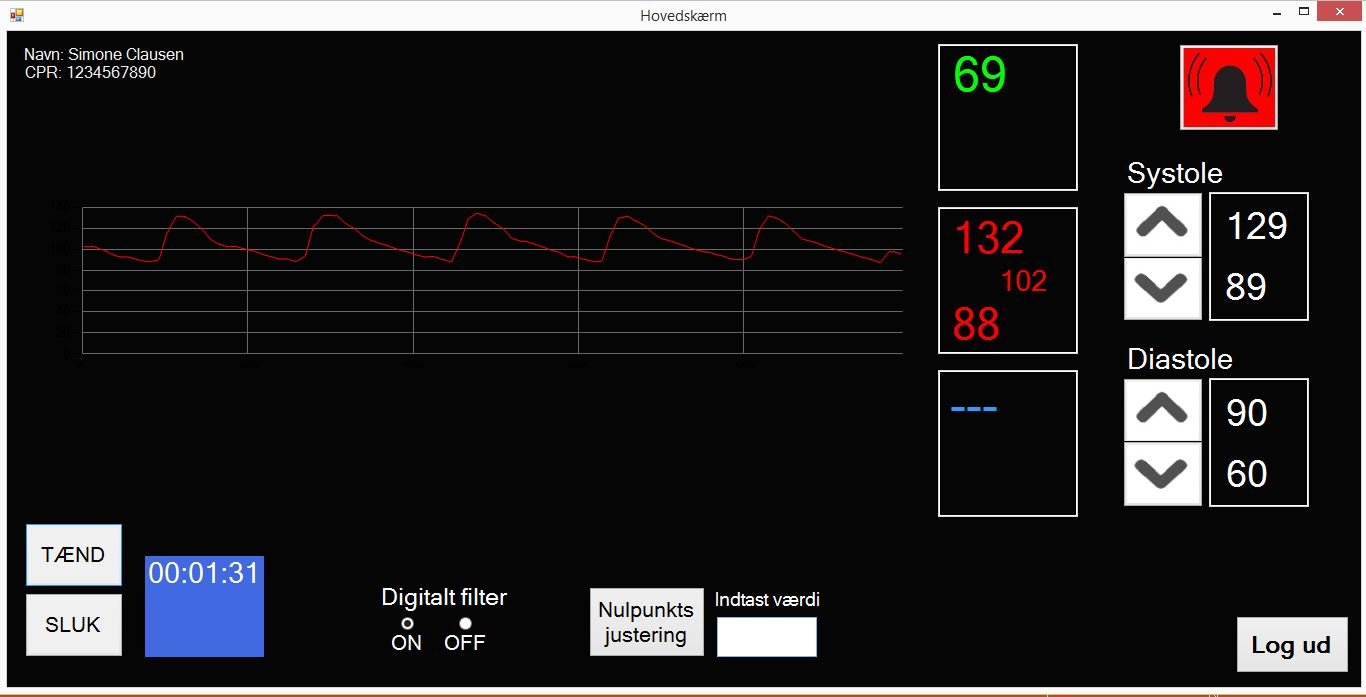
\includegraphics[width =0.6\textwidth , center]{billeder/IThovedGUIAlarm}
\caption{\textbf{Grænseværdi for systole ændret og alarm igangsat.}}
\end{figure}
I acceptesten for Use case 4, skal der trykkes på sluk, derefter log ud og til sidst ja på pop-up vinduet. På figuren neden for, ses der at der er trykket på sluk-knappen, da den er blevet gennemsigtig, og kun tænd-knappen der kan trykkes. Log ud er blevet trykket for at bekræft pop-up vinduet er kommet frem. Herved virker log ud knappen som den skal, og der bliver gemt målingen for patienten i EPJ-databasen. Blodtryksmålingen for patienten bliver gemt løbende i EPJ-databasen. 
\begin{figure}[H]
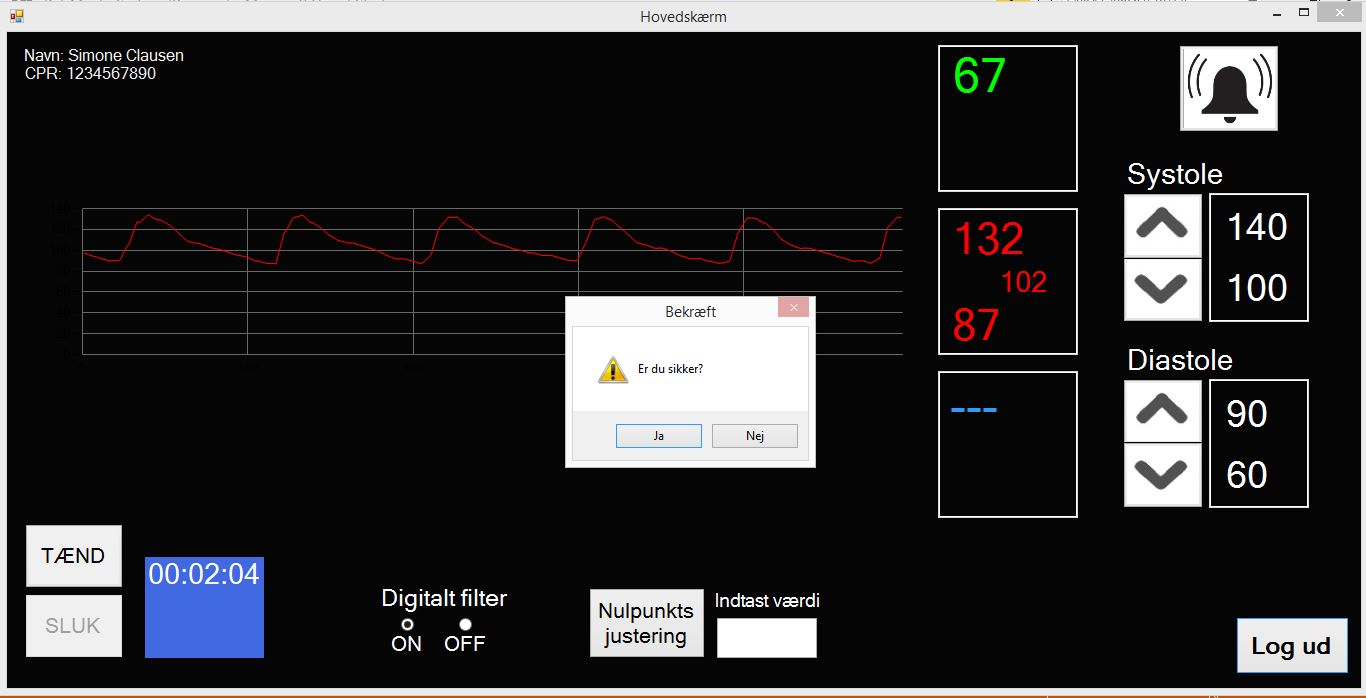
\includegraphics[width =0.6\textwidth , center]{billeder/IThovedGUILogUd}
\caption{\textbf{Log ud af blodtryksmålersystemet.}}
\end{figure}
Fra de foregående figur kan det konkluderes at blodtryksmålersystemet lever op til accepttestens krav omkring, at kunne vise et blodtrykssignal kontinuert, samt slå et digitalt filter til og fra. \\\\
Blodtryksmålesystemet lever også op til kravet omkring at kunne kalibrere systemet. Dette gøres på startskærmen. Kravet til at systemet kan nulpunktsjusteres er ligeledes opfyldt, denne sker på hovedskærmen. Det kan diskuteres om det var smartere at systemet selv skal kunne indlæse værdien for nulpunktjustering, og derefter bare lægge denne denne værdi til blodtrykssignalet, når der trykkes på nulpunktsjusterings knappen, end at man selv skal aflæse værdien. Dog lever nulpunktsjusterings knappen, op til kravet omkring at nulpunktsjustere blodtryksmålesystemet, da alle blodtrykssignalværdierne bliver nulpunktsjusteret efter den indtastet nulpunktsværdi. \\\\
Grænseværdierne for blodtryksmålesystemet kan også ændres, herved er dette krav opfyldt, og der kommer en alarm når værdierne for enten systolen eller diastolen overskrider de satte grænseværdier. \\
Alarmen kan også udsættes i et minut, hvilket gøres ved at trykke på alarmknappen oppe i højre hjørne af hovedskærmen. \\\\
En anden ting som blodtryksmålersystemet også kan er at vise en timer, som starter når man har trykket på start knappen, og stopper når der trykkes på sluk knappen. Det kan diskuteres hvor smart det er, om timeren skal nulstille, når der trykkes på start knappen igen. Der er valgt i dette projekt at timeren starter fra det stoppet tidspunkt, når tænd bliver trykket igen, dette er valgt fordi, at det giver bedst mening at man skal kunne starte fra hvor man slap. Dog giver den funktion med at starte timeren igen, ikke så meget mening ude i den virkelige verden, da anæstesi sygeplejerskerne ikke starter målingen igen, efter at have stoppet målingen. \\\\
Det kan diskuteres om brugeren skal have lov til at kalibrer på startskærmen, da kalibrering skal fortages af en servicemedarbejder. Herved skulle der kun have været log ind på startskærmen, og være lavet et servicevindue, som kun kan betjenes af servicemedarbejderen. Der er taget højde for denne problemstilling i koden, ved at have lavet en config fil, hvor kalibreringstallet kan ændres. Det betyder, at hvis det sundhedsfagligt personale springer over at kalibrere på startskærmen kalibrerer systemet automatisk efter kalibreringstallet i config filen. Meningen med config filen, er at det kun er servicepersonalet der skal kunne tilgå denne fil, og kunne ændre kalibreringstallet. 
\section{Udviklingsværktøjer}
Til udviklingen af produktet, og dermed igennem hele projektarbejdet, er der blevet brugt en række udviklingsværktøjer. I dette afsnit er disse udviklingsværktøjer beskrevet yderligere.
\subsection{Microsoft Visio 2010}
Tegneværktøjet Microsoft Visio, er blevet anvendt i forbindelse med design af både UML og SysML diagrammer. Microsoft Visio er det oplagte valg til at designe disse diagrammer, da programmet søger for at diagrammerne får et enkelt udseende og tydeligt kommunikerer til læseren, hvad diagrammerne vil vise.
\subsection{Visual Studio 2013}
Visual Studio 2013 er et udviklingsværktøj, designet til Microsoft .Net-frameworket. Dette udviklingsværktøj er specielt velegnet til design af brugergrænseflader, som i dette projekt er specifikt brugbart, da der skal udarbejdes et Windows Forms program.
\subsection{NI Multisim 13.0 med Ultiboard 13.0}
Til at designe hardwaren er Multisim med Ultiboard blevet benyttet. Multisim er et program der kan bruges ved kredsløbsdesign, da komponenterne her er lette at sætte i forhold til hinanden, da programmet indeholder samtlige komponenter. Ultiboard bruges til at designe printet, der skal bruges til at realisere hardwaren, der er blevet designet i Multisim. Ved at benytte Ultiboard undgås det at benytte et fumlebræt eller veroboard, hvor komponenterne skal kobles sammen med ledning. Ved et print der designes med Ultiboard vil forbindelserne mellem komponenterne være direkte implementeret på pritet og komponenterne vil derfor være nemme at implementere på printet.
\subsection{NI-DAQmx}
NI-DAQmx, også omtalt NI-DAQ/DAQ, er et værktøj som er blevet udarbejdet af National Instrument. Dette værktøj anvendes til at indsamle det indkommende signal. Dette signal kommer fra hardwaren. NI-DAQ omdanner desuden signalet fra et analogt signal til at være et digitalt signal der kan bruges i koden. 
\subsection{Analog Discovery fra Digilent and Analog Devices}
Analog Discovery er i projektet den der benyttes om en waveform-generator. Det er derfor Analog Discovery der benyttes til at teste systemet. Dette sker ved at der sendes et blodtrykssignal fra Physionet.org ind i systemet, som systemet derefter skal behandle. Desuden er oscilloskopfunktionen i waveforms blevet benyttet under test af hardware.
\section{Opnåede erfaringer}
På baggrund af vores sundhedsfaglige viden og de opsatte rammer for projektet, er der blevet opstillet en projektformulering, som er løst ved hjælp af viden omkring programmering, analog og digital signalbehandling, SysML og UML. Arbejdet har styrket vores tværfaglige kompetencer og vi har formået at skabe en teknisk løsning på et sundhedsfagligt problem.\\
Kompetencerne inden for digital signalbehandling, er indenfor dette projekt opnået ved at udarbejde et moving average lavpasfilter. Inden det blev klart at dette lavpasfilter skulle benyttes, er flere forskellige filtre blevet afprøvet. Disse filtre er ved brug af programmet MatLab blevet afprøvet, et butterworth IIR (Infinite impulse filter) lavpas filter her blev udarbejdet. Det var dog et FIR (Finite impulse filter) lavpasfilter der skulle benyttes, hvilket førte frem til at moving average filteret blev afprøvet, hvilket virkede efter hensigt. \\
Programmerings koden til filteret skulle herefter udarbejdes, her blev der undersøgt forskellige metoder der kunne benyttes via søgninger på internettet, hvilket sammen med at "snakke og tegne" koden førte frem til at koden kunne skrives til det digitale filter. Realiseringen af lavpasfilteret forbedrede derfor ligeledes programmeringskompetencerne. Det at "snakke og tegne" koden, blev brugt ved alle problemstillingerne i programmeringen, for at finde frem til den tilgang der skulle bruges for at løse problemet. Bl.a. ved udarbejdelse af metoden til hvordan der skulle holdes styr på den data der skulle sendes op, blev koden "snakket og tegnet" igennem inden. Idet blodtrykket skulle vises løbende, skulle der være en kømetode, som kunne indhente og udsende data løbende og samtidig holde styr på data i køen.\\
Andre software kompetence er ligeledes blevet opnået, ved at benytte forskellige mønstre og kode opbygninger, hvor netop kombinationen af disse faktorer har ført til en bredere forståelse i programmering og hvordan et projekt logisk kan bygges godt op. Herunder hvor de forskellige metoder må ligge og hvordan klasserne må snakke sammen. \\\\
Data der skulle sendes ind i kodes, skulle først igennem den udarbejdede hardware. Under udarbejdelsen af hardware produktet er kompetencerne inden for analog signalbehandling, blevet forbedret. Ud fra problemstillingen og projektformuleringen vidste vi hvordan signalet skulle sendes ind, her skulle kredsløbet, der skulle praktisere dette, først designes. En forstærker og et lavpasfilter skulle designes, hvilket blev gjort i forskellige fase, først igennem forskellige beregninger, som kunne føre til at bestemme komponenterne der skulle benyttes ved forstærkeren og lavpasfilteret. Herefter kunne kredsløbet designes i multisim og på fumlebræt for at se om det analyserede kredsløbet kunne realiseres. \\\\
Det var lærerigt at give reviews til andre grupper, da vi her fik muligheden for at reflektere over, hvordan vi selv havde arbejdet med projektet og samtidig fik vi et indblik i, hvordan de andre grupper havde valgt at gribe opgaven an. Der blev udført to reviews, et review på kravspecifikation og accepttest og et review på design og specifikation af software og hardware.  Desværre har der gennem projektforløbet været en del forvirring på tværs af grupperne omkring diverse krav og fremgangsmåder vedrørende projektudførelsen, hvilket gjorde review møderne mindre udbytterige end de kunne have været.\\\\
Projektstyringen og ledelsen må vi indse har været for svag i dette projekt. Rigtigt ville vi have benyttet SCRUM, men dette kom ikke rigtig op og køre, så opgaverne har været mere løst opsatte. Hvor vi igennem SCRUM kunne have haft identificeret mere klare opgaver og sætte en fast deadline for, hvornår opgaven skulle være færdig. Ligeledes kunne opgaverne her prioriteres sådan det også blev identificeret hvor stor opgaven er og hvor høj prioritering denne opgave har. Det må dog også erkendes at fordelingen af ressourcerne ikke har været optimalt. 
\section{Fremtidigt arbejde}
I dette projekt har der været flere overvejelser om hvorledes vi ønskede vores slutprodukt skulle se ud og hvilke funktioner vi efterstræbte at opfylde. Vores besøg på Herning sygehus gav os et indblik i hvordan en invasiv blodtryksmåler fungerer i praksis og hvilke funktioner der er indbygget heri. Vi ønskede altså at basere vores system ud fra et virkeligt brugsscenarie. Dette brugte vi som udgangspunkt for vores system og vi udtænkte derfor en ide og opstillede et design, som vi ville udarbejde i vores projekt. Vores produkt skulle slutteligt kunne vise både EKG, systolisk samt diastolisk blodtryk og iltmætning. Alle værdier skulle udskrives i en graf og talværdierne vises på brugergrænsefladen. 
\subsection{EKG-signal}
EKG-signalet skulle  simuleres ved at sende et EKG-signal fra physionet.org via analog discovery ind i en anden port i DAQ’en, dette signal skulle så på lige fod med blodtryks-data præsenteres visuelt. Ligeledes skulle der være mulighed for at disse data kunne gemmes i databasen.
\subsection{Iltmætning}
Iltmætning ønskede vi at implementere i vores system, så dette, ligeledes som blodtrykket og EKG, ville blive præsenteret visuelt. For at få vist iltmætning ville vi benytte et pulsoxymeter. Pulsoxymeteret sættes på fingeren og virker ved at gennemlyse fingeren med infrarødt lys. Herved måles iltmætningen i blodet. Disse data kunne via USB overføres til programmet. 
\subsection{EPJ}
Fremtidigt ville vi implementere vores system op mod eksisterende EPJ systemer, da vores system allerede er baseret på et virkeligt brugsscenarie, forventer vi at en implementation ville være relativt enkel. Vores patientdata ville i stedet for vores database være hentet fra EPJ.  Ligeledes vil vores logindata for plejepersonalet være hentet enten i Active Directory (netværket) eller i medarbejderdatabasen. Blodtryksdata vil stadig skulle gemmes separat, men som vi kommer ind på i næste afsnit omkring datawarehouse, så skal data være kvalificeret af en række metadata.
\subsection{Datawarehouse}
Det blev fra projektets start talt om at lave et datawarehouse, realiseret med et slags mock-up datawarehouse til analysering af blodtryksmålinger. Et datawarehouse er en samling af data fra forskellige kilder, der er sorteret efter emne, i vores tilfælde ville det være eksempelvis være blodtryksmåledata. Dette emne ville så være kvalificeret af en række dimensioner, som vil være repræsenteret af metadata i vores database.\\ 
Metadata / dimensioner kunne være ting som:
\begin{itemize}
\item Aldersgruppe eller alder
\item Køn
\item Datotid
\item SKS-koder (Sundhedsvæsnets Klassifikations System)
\item Behandlingssteder/Afdelinger
\item Andre metadata fra EPJ
\end{itemize}
Et datawarehouse fungerer absolut bedst når der er akkumuleret mange data, da det giver et mere retvisende billede af tendenser. 
\chapter{Konklusion}
- Line
Afrunding
konkludering
Hvad lykkedes og hvad lykkedes ikke